\chapter{Projektorganisation}

\section{Vorgehen}
Das Projekt wurde in den Grunds�tzen an den RUP\footnote[1]{Rational Unified Process: \href{https://de.wikipedia.org/wiki/Rational\_Unified\_Process}{https://de.wikipedia.org/wiki/Rational\_Unified\_Process}} Prozess angelegt. Als wichtigstes Merkmal wurden die Projektphasen Inception, Elaboration, Construction 1, Construction 2, Construction 3 und Transition definiert.

\section{Risiken}
W�hrend des Projektes wurde festgestellt, dass die ASD Implementierung Eigenheiten besitzt, welche am Anfang untersch�tzt wurden. Deshalb wurde eine Risikoanalyse vorgenommen und die Risiken des Projektes abgesch�tzt. Die Risikobewertung wurde jeweils beim �bergang in eine neue Phase vorgenommen. Im folgenden Kapitel sind die Hauptrisiken aufgelistet.

\subsection{ASD Dokumentation stimmt nicht mit Realit�t �berein}
Als Hauptrisiko mussten wir feststellen, dass die ASD Dokumentation nicht korrekt oder schwierig interpretierbar ist. Dieses Risiko ist eingetroffen. Als Massnahme wurde Code externer Entwickler und vom Kunden in Anspruch genommen, um die Daten besser interpretieren zu k�nnen.
\begin{figure}[h]
	\begin{center}
		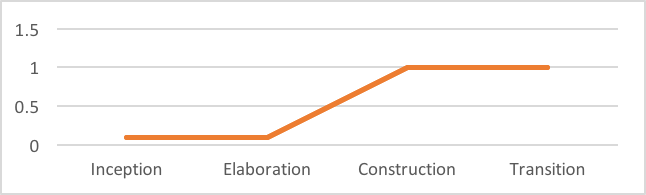
\includegraphics[scale=1]{images/Risk1} 
	\caption{Risikoverlauf "ASD Dokumentation"}
	\label{fig:risk1}
	\end{center}
\end{figure}

\subsection{Zu wenig Zeit um alle Anforderungen zu erf�llen}
Dieses Risiko wurde von Anfang an bewusst angegangen. So wurden bereits w�hrend der Anforderungserhebung eine Priorisierung der einzelnen Punkte vorgenommen. Dieser Prozess erfolgte in Zusammenarbeit mit dem Kunden. Dadurch konnte dieses Risiko minimiert werden.
\begin{figure}[h]
	\begin{center}
		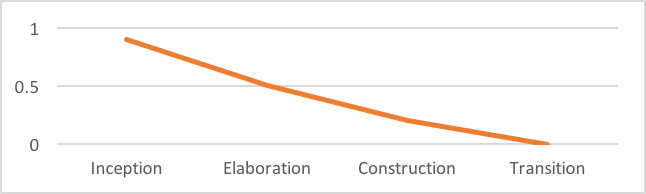
\includegraphics[scale=1]{images/Risk2} 
	\caption{Risikoverlauf "Zeit"}
	\label{fig:risk2}
	\end{center}
\end{figure}

\subsection{Daten vom iOS Ger�t importieren und exportieren}
Dieses Risiko bestand, da im Gegensatz zu vielen etablierten Apps einige Dateien zwingend f�r das Funktionieren der Applikation bereits zu Beginn bereitgestellt werden m�ssen. Die Sorge war, keine einfache Methode anbieten zu k�nnen, um einfach und intuitiv Daten auf das iPad zu kopieren. Dieses Risiko konnte ausger�umt werden, indem Nachforschungen zu bekannten Apps, welche diese Problemstellung gel�st hatten, intensiviert wurden. Es wurde festgestellt, das iOS bereits eine eigene elegante L�sung f�r diesen Prozess bietet, welcher nun auch verwendet wird. Das Importieren wird in Punkt \ref{sec:iosApp} beschrieben.
\begin{figure}[h]
	\begin{center}
		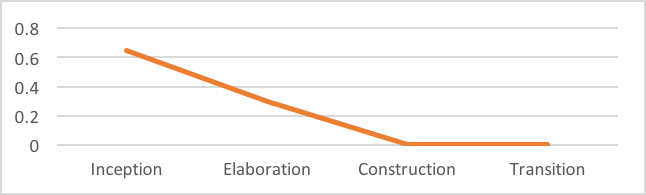
\includegraphics[scale=1]{images/Risk3} 
	\caption{Risikoverlauf "Import und Export"}
	\label{fig:risk3}
	\end{center}
\end{figure}

\section{Meilensteine}
Die Meilensteine wurden ebenfalls an den RUP Prozess angelegt und sind so meist bei den �berg�ngen in die n�chste Phase definiert. In der nachfolgenden Tabelle sind die definierten Meilensteine des Projektes nach Datum geordnet:

\begin{center}

	\bgroup
	\def\arraystretch{1.5}
    \begin{tabular}{ | c | l | p{13cm} |} \hline
    
    \textbf{Nr.} & \textbf{Datum} & \textbf{Beschreibung} \\ \hline
    
    001 & 23.10.2016 & \textbf{Einlesen und Spektrometer�bergabe} \newline
    Die Spektrometer konnten von den Studierenden in Empfang genommen werden. \\ \hline
    
    002 & 30.11.2016 & \textbf{Anforderungen} \newline
    Das Pflichtenheft wurde erstellt und vom Kunden akzeptiert. \\ \hline
    
    003 & 30.11.2016 & \textbf{Proof of Concept} \newline
    Es liegt ein funktionierender Proof of Concept vor, der die Verbindung zum Spektrometer herstellen und Antworten empfangen kann. \\ \hline
    
    004 & 21.12.2016 & \textbf{Prototyp 1} \newline
    Ein funktionierender Prototyp mit allen Anforderungen der Priorit�t 1 ist f�r den Kunden im TestFlight freigegeben. \\ \hline
    
    005 & 25.01.2017 & \textbf{Prototyp 2} \newline
    Ein funktionierender Prototyp mit allen Anforderungen der Priorit�t 2 ist f�r den Kunden im TestFlight freigegeben. \\ \hline
    
    006 & 01.03.2017 & \textbf{Version 1.0} \newline
    Eine funktionierende Version der App mit allen Anforderungen der Priorit�t 3 ist f�r den Kunden im TestFlight freigegeben. \\ \hline
    
    007 & 16.03.2017 & \textbf{Projektabschluss} \newline
    Die finale Version mit allen Fehlerverbesserungen aus Version 1.0 ist im TestFlight f�r den Kunden freigegeben. \\ \hline
    
    \end{tabular}
    \egroup
    
\end{center}

\section{Zeitplanung}
Die Zeitplanung wurde mithilfe der RUP Phasen durchgef�hrt. Damit konnte die Dauer der einzelnen Phasen abgesch�tzt und mit den Meilensteinen abgestimmt werden. Es musste noch auf einige Abwesenheiten des Kunden geachtet werden. Die Meetings f�r die Prototyp Pr�sentation mussten somit etwas vor- oder nach den jeweiligen Releasedaten der Prototypen angesetzt werden. Der Zeitplan befindet sich in detaillierter Form auch im Anhang.

\begin{figure}[h]
	\begin{center}
		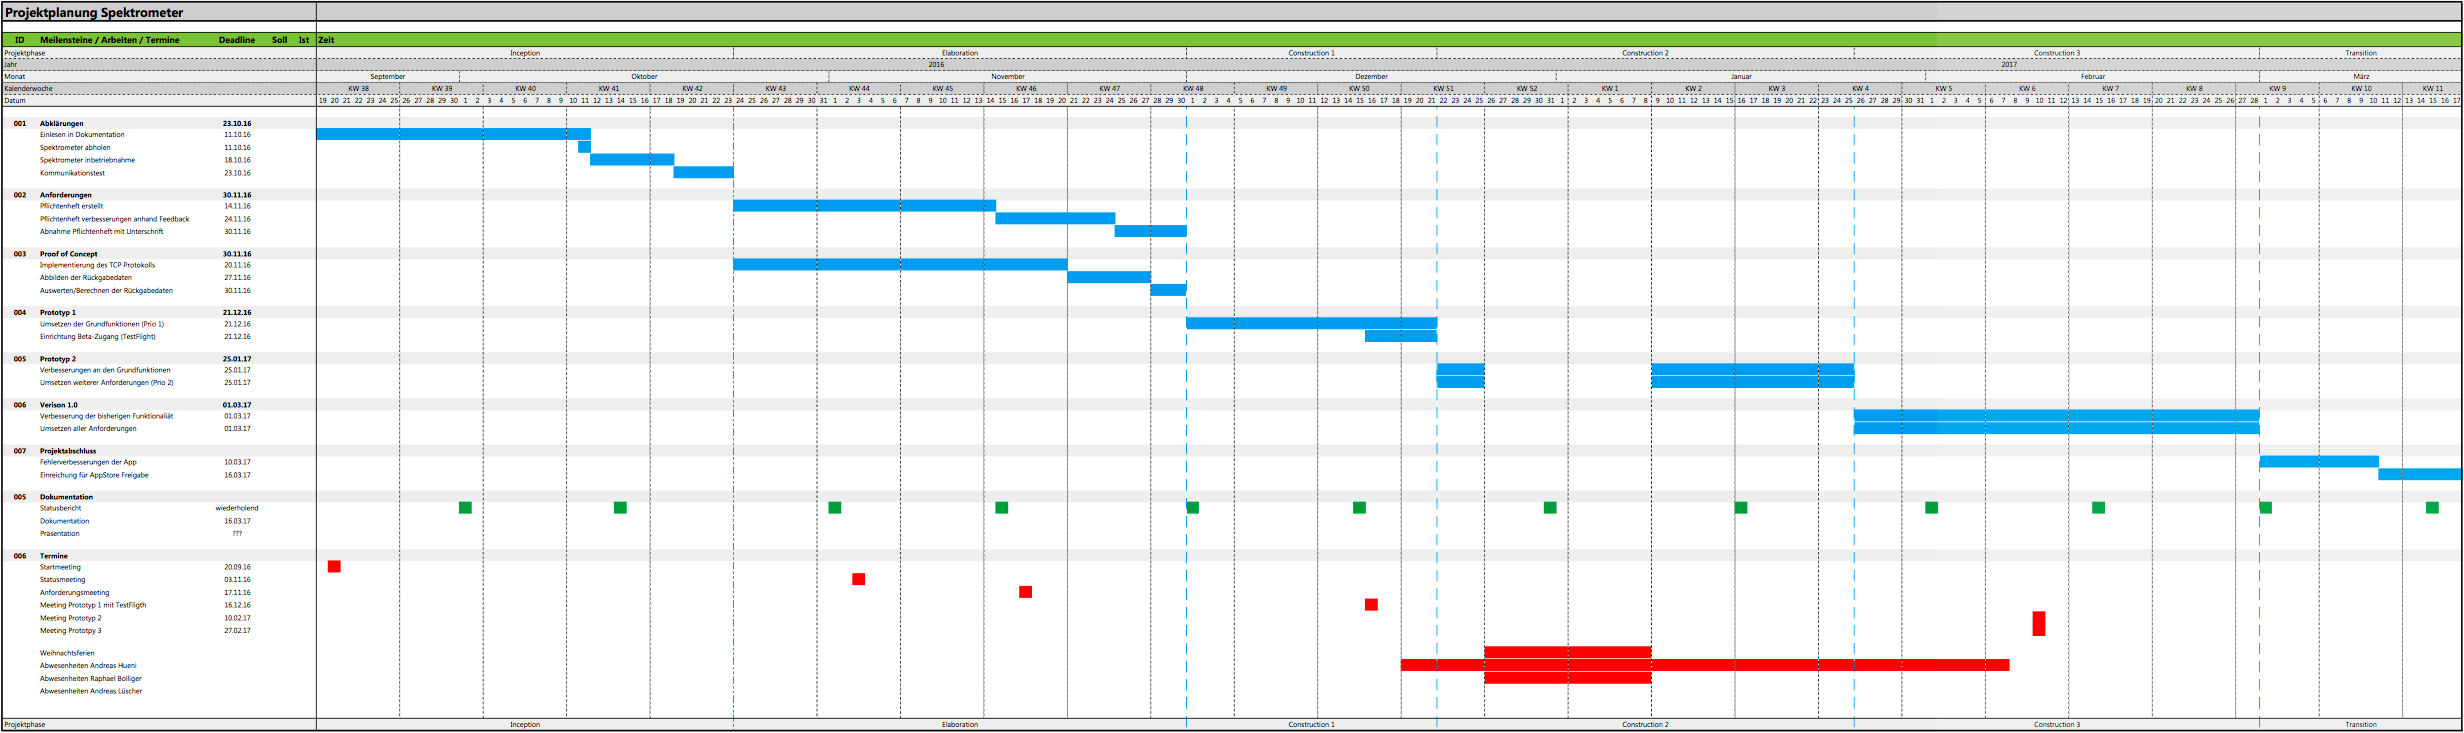
\includegraphics[scale=0.19]{images/TimePlanning} 
	\caption{Zeitplanung}
	\label{fig:TimePlanning}
	\end{center}
\end{figure}

\section{Anforderungen}
Die Anforderungen wurden zu Beginn bei einem Startmeeting mit dem Kunden besprochen. Weiter konnten viele Anforderungen detailliert in der bestehenden Software ausgemacht werden. Die Anforderungen wurden in einem Pflichtenheft zentral erfasst und priorisiert. Die Priorit�ten markieren zudem, in welchem Prototyp eine Anforderung umgesetzt wurde. Anforderungen mit der Priorit�t 4 wurden nicht zwingend umgesetzt, diese haben keinen Einfluss auf die Funktionalit�t der neuen Applikation. Detaillierte Informationen zu den Anforderungen sind im Anhang zu entnehmen.

\section{Change Management}
Die Anforderungen haben sich bis kurz vor Projektende nie ge�ndert. Nach dem Einreichen der Version 1.0 kam die Anforderung dazu, den Dark Current mit einer Konfigurationsdatei zu hinterlegen sowie zu Berechnen. Da diese so kurzfristig war, konnte sie nicht mehr innerhalb der Projektzeit umgesetzt werden.

Auf ein Change Management wurde bewusst verzichtet, da sich nach Projektstart abzeichnete, dass die Anforderungen genug detailliert und vollst�ndig erfasst wurden.

\section{Arbeitspakete}

Da die Anforderungen sehr detailliert unterteilt wurden, dienten sie zugleich als Arbeitspakete. Eine Anforderung konnte so meist von einer Person implementiert werden.

\section{Soll- und Istvergleich}